\documentclass{article}
\usepackage{graphicx}
\usepackage{amsthm}
\theoremstyle{definition}
\newtheorem{example}{Example}

\title{The Airport Commute Problem}
\author{Iva Babukova}
\date{July 2016}

\begin{document}
\maketitle
In this work we present the Traveler's Problem (TP), a computational task whose extensions and variations are often encountered by travelers around the world. The task is concerned with creating a valid travel schedule, using airplanes as a means of transportation and in accordance with certain constraints specified by the traveler.

Each instance of TP consits of:

\begin{enumerate}
\item A set of airports. Airports represent locations a traveler can begin their commute in, visit as a desired destination, or connect in on the way to their destination.
\item A set of flights. Each flight includes arrival and departure airports, as well as a price and a date.
\item The starting point, which is a single airport chosen from the set of airports
\item A set of destinations the traveler wants to visit, which is a subset of the set of airports.
\end{enumerate}

A solution to any instance of TP is a sequence $s$ of valid flights, ${f_{1}, f_{2}, ..., f_{k}}$. We say that a sequence contains valid flights if the flights in the sequence have the following properties:

\begin{enumerate}
\item The departure airport of the first flight in $s$, $f_{1}$, is equal to the arrival airport of the last flight in $s$, $f_{k}$ is equal to the starting point.
\item For any two consecutive flights in $s$: $f_{i}$, $f_{i+1}$, we have that the arrival airport of $f_{i}$ is equal to the departure airport of $f_{i+1}$
\item The flights in $s$ have dates, which occur in increasing, temporal order (flights earlier in the list happen earlier in time).
\item All destinations the traveler wants to visit are included in at least one flight from $s$.
\end{enumerate}

An optimal solution is a solution, which minimises the total sum of flight's prices.

Any solution (including any optimal solution) may include airports a traveler has not specified on their list of destinations. Such airports are called connections.

We note that the specification of TP as presented above may not reflect requirements of many travelers. Indeed, travelers may have additional preferences (soft contstraints) and requirements (hard constraints) with regards to their travel. For example, travelers may require to spend a minimum number of days in a given destination, or trade off an additional day at a destination for increase in total travel price. Travelers may require to spend a given date at a given destination, for example due to an event occuring on that date in this destination. Additionaly, connections may be penalised by some users, perhaps with penalty proportional to the waiting time. The traveler may have a certain price threshold (budget), such that if the total travel cost exceeds that threshold the traveler will discard a solution as invalid.

It is therefore suggested that any attempt at an investigation of TP assumes as an additional non-functional requirement, that any proposed model to solve TP is flexible and can be easily extended by adding, removing and modifying soft and hard constraints.

\begin{figure}[h]
\centering
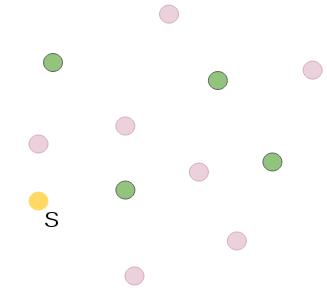
\includegraphics[width=5cm, height=4cm]{destinations0.png}
\end{figure}

TP is interesting both practically and theoretically. We therefore give two presentations of the same instance of the problem. One in form of a user story, which should be familiar to many software engineers, and one stated more formally, targeted at algorithmicians.

\begin{example}
Adam lives in Glasgow and he will be on holiday for two weeks, starting from the 1st of August. He wants to find the cheapest way to visit Milano, Berlin, Amsterdam and Paris by plane. Adam wants to spend no less than 3 days in each city and does not have any preference on the order in which he visits cities. %However, there are particular events which Adam does not want to miss out. In particular, on 5th of August there is a bierfest in Berlin and on 10th of August there is a festival in Paris.
Adam can start his trip from the evening on 31st of August and he must be back to Glasgow by the evening on 14th of August. Adam does not have any preferences on the choice of airline company.
\end{example}

\end{document}







